\documentclass[11pt,a4paper]{article}
\usepackage[utf8]{inputenc}
\usepackage[T1]{fontenc}
\usepackage{amsfonts}
\usepackage[french]{babel}
\frenchbsetup{StandardLists=true}
\usepackage{enumitem}
\usepackage{amssymb}
\usepackage{amsmath}
\usepackage[left=1.5cm,right=1.5cm,top=2cm,bottom=2cm]{geometry}
\usepackage{multirow}
\usepackage[dvipsnames]{xcolor}
\usepackage{fouriernc}
\usepackage{setspace}
\singlespacing
\setlength{\parindent}{0pt}
\usepackage{multicol}
\setlength{\columnseprule}{1pt}
\usepackage{pstricks}
\usepackage{tikz}
\usepackage{pst-labo}
\usepackage{graphicx}
\usepackage{fancyhdr}
\pagestyle{fancy}
\renewcommand\headrulewidth{1pt}
\fancyhead[L]{Lycée Denis Diderot }
\fancyhead[R]{Classe de 1 Bac Pro}
\setcounter{page}{1}\fancyfoot[C]{page \thepage}
\fancyfoot[R]{Année 2025-2026}
\fancyfoot[L]{Alexis RUIZ}
\usepackage{multirow,tabularx,booktabs}
\usepackage{array}
\begin{document}
\hrule
\vspace{3mm}
\center \LARGE{Annexe 1 : Identification de la verrerie de laboratoire}\\[0,6cm]
\hrule
\normalsize
\vfill
\textbf{Consigne :} Identifier chaque ustensile de verrerie et écrire son nom dans la case correspondante.
\vfill
\definecolor{GrisClair}{rgb}{0.8,0.8,0.8}
\newpsstyle{aspectLiquide1} {linestyle=none,fillstyle=solid,fillcolor=GrisClair}
% Tableau 4x5 = 20 cases avec pst-labo
\begin{center}
\begin{tabular}{|c|c|c|c|c|}
\hline
% Ligne 1
\psset{unit=0.6cm}
\pstTubeEssais
&
\psset{unit=0.6cm}
\pstTubeEssais[glassType=becher]
&
\psset{unit=0.6cm}
\pstTubeEssais[glassType=erlen]
&
\psset{unit=0.6cm}
\pstTubeEssais[glassType=ballon]
&
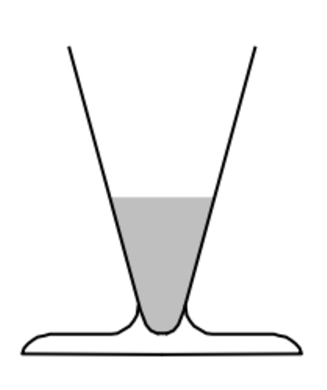
\includegraphics[height=2.5cm]{images/verre.eps} \\[0.2cm]
\framebox[2.5cm][c]{\rule{0cm}{0.8cm} \raisebox{3mm}{\textcolor{red}{Tube à essais}}} &
\framebox[2.5cm][c]{\rule{0cm}{0.8cm} \raisebox{3mm}{\textcolor{red}{Bécher}}} &
\framebox[2.5cm][c]{\rule{0cm}{0.8cm} \raisebox{3mm}{\textcolor{red}{Erlenmeyer}}} &
\framebox[2.5cm][c]{\rule{0cm}{0.8cm} \raisebox{3mm}{\textcolor{red}{Ballon}}} &
\framebox[2.5cm][c]{\rule{0cm}{0.8cm} \raisebox{3mm}{\textcolor{red}{Verre à pied}}} \\[0.2cm]
\hline
% Ligne 2
\raisebox{-23mm}{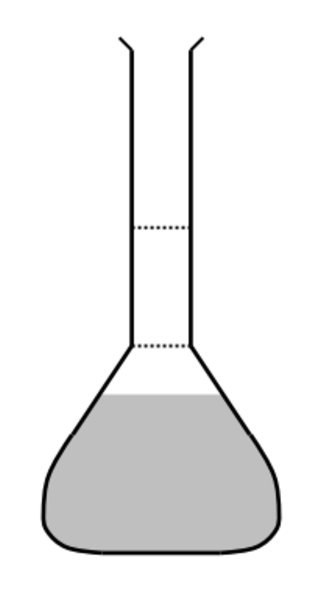
\includegraphics[height=3.5cm]{images/fiole.eps}}
&
\multicolumn{2}{|c|}{\raisebox{-2.7cm}{\psset{unit=0.5cm} \pstChauffageBallon[glassType=ballon,recuperationGaz,tubeRecourbeCourt]}}
&
\raisebox{-18mm}{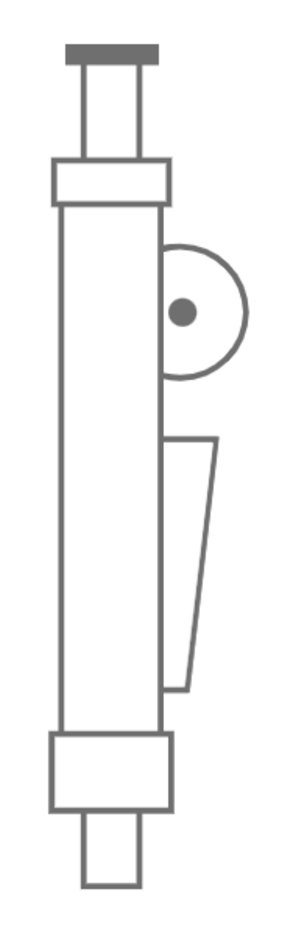
\includegraphics[height=3.5cm]{images/propipette.eps}}
&
\raisebox{-18mm}{\begin{tikzpicture}[scale=0.8, thick, line width=1pt]
% Ellipse du haut
\draw (0,2.7) ellipse (1.2 and 0.2);
% Côtés droits
\draw (-1.2,2.7) -- (-0.15,1.5);
\draw (1.2,2.7) -- (0.15,1.5);
% Tube central (plus long)
\draw (-0.15,1.5) -- (-0.15,0);
\draw (0.15,1.5) -- (0.15,0);
% Bout du tube
\draw (-0.15,0) .. controls (0,-0.05) .. (0.15,0);
\end{tikzpicture}} \\[2cm]
\framebox[2.5cm][c]{\rule{0cm}{0.8cm} \raisebox{3mm}{\textcolor{red}{Fiole jaugée}}} &
\multicolumn{2}{|c|}{\framebox[4.5cm][c]{\rule{0cm}{0.8cm} \raisebox{3mm}{\textcolor{red}{ Récupérateur de gaz}}}} &
\framebox[2.5cm][c]{\rule{0cm}{0.8cm} \raisebox{3mm}{\textcolor{red}{Propipette}}} &
\framebox[2.5cm][c]{\rule{0cm}{0.8cm} \raisebox{3mm}{\textcolor{red}{Entonnoir}}} \\[0.2cm]
\hline
% Ligne 3
\raisebox{-14mm}{
\includegraphics[height=3cm]{images/chauffe.eps}}
&
\raisebox{-1.2cm}{\psset{unit=0.5cm}
\pstDosage[glassType=erlen,burette=false]}
&
\multirow{2}{*}{\raisebox{100mm}{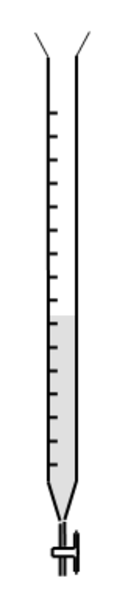
\includegraphics[height=6.3cm]{images/burette.eps}}}
&
\multirow{2}{*}{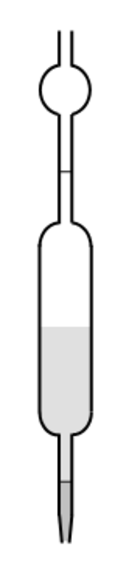
\includegraphics[height=6.3cm]{images/pipette.eps}}
&
\multirow{2}{*}{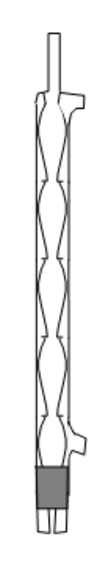
\includegraphics[height=6.3cm]{images/refrigerant.eps}}
\\[1cm]
\framebox[2.7cm][c]{\rule{0cm}{0.8cm} \raisebox{3mm}{\textcolor{red}{Chauffe-ballon}}} &
\framebox[2.5cm][c]{\rule{0cm}{0.8cm} \raisebox{3mm}{\textcolor{red}{Erlenmeyer}}} &
&
&
\\[0.2cm]
\cline{1-2}
% Ligne 4
\multicolumn{2}{|c|}
{\raisebox{-1.4cm}{\psset{unit=0.7cm,glassType=becher,burette=false}
\pstDosage[phmetre]}}
&
&
&
\\[1.5cm]
\multicolumn{2}{|c|}{\framebox[4.5cm][c]{\rule{0cm}{0.8cm} \raisebox{3mm}{\textcolor{red}{pH-mètre}}}} &
\framebox[2.5cm][c]{\rule{0cm}{0.8cm} \raisebox{3mm}{\textcolor{red}{Burette}}} &
\framebox[2.5cm][c]{\rule{0cm}{0.8cm} \raisebox{3mm}{\textcolor{red}{Pipette}}} &
\framebox[2.5cm][c]{\rule{0cm}{0.8cm} \raisebox{3mm}{\textcolor{red}{Réfrigérant}}} \\[0.2cm]
\hline
\end{tabular}
\end{center}
\vfill
\end{document}
